\chapter{Detalles de Implementación y Experimentos}
\label{chapter:implementation}
El objetivo de esta tesis es comparar dos de las heuristicas integradas a CDCL, en este caso, dos de las que intentan dar soluci\'on al problema de selecci\'on de variables: Dichas estrategias, VSIDS y DLIS, son comparadas usando \textit{restart} y no.

En el trabajo se usaron los lenguajes de programaci\'on C++, Python y bash. CaDiCaL est\'a programado en C++, por lo que es el lenguaje en el que est\'an implementadas las heur\'isticas. Python fue usado para automatizar los procesos de pruebas, guardar los resultados obtenidos y realizar los an\'lisis estad\'sticos. Finalemnte, bash se usa como parte de la ``compilaci\'on'' del solver, cuyos archivos como \textit{configure} y \textit{makefile} que vienen integrados al \textit{solver}, son los encargados de hacerlo funcionar.

\subsection{CaDiCaL}
CaDiCaL fue el \textit{solver} escogido para esta comparaci\'on, ya que cuenta con la posibilidad de activar y desactivar VSIDS (ya viene integrada), al igual que la estrategia \textit{restart}, tambi\'en integrada en el solucionador.\footnote{Cabe destacar que CaDiCaL ofrece esta misma posibilidad para much\'isimas heur\'isticas, adem\'as de estrategias para adaptar la v\'ia de soluci\'on al tipo de problemas [\cite{cadical2024}]} Como ya se mencion\'o con anterioridad en este documento, pr\'acticamente todos los CDCL SAT \textit{solvers} modernos no incluyen DLIS como heur\'istica de selecci\'on de variables, y CaDiCaL es uno de ellos. Por esta raz\'on, se decidi\'o integrar una implementaci\'on de DLIS a este solucionador, aprovechando la pol\'itica \textit{open source} de su c\'odigo fuente [\cite{cadical2024}].%insertar link al repo original de cadical.

\subsubsection{Integraci\'on de DLIS}
Para integrar DLIS en CaDiCaL se modificaron los siguientes archivos:
\begin{itemize}
    \item \textit{internal.hpp}
    \item \textit{internal.cpp}
    \item \textit{decide.cpp}
    \item \textit{options.hpp}
\end{itemize}

{\textit{internal.hpp}}
En este archivo se declaran los m\'todos que se implementaron como parte de la clase \textit{Internal} \ref{lst:cadical-dlis-internal.hpp}:

\begin{lstlisting}[
    language=C++,
    caption={Integracion de DLIS en CaDiCaL. Internal.hpp},
    label={lst:cadical-dlis-internal.hpp},
    captionpos=b,
    frame=tb
]
// DLIS
int next_decision_variable_with_dlis ();
int count_literal_in_unsatisfied_binary_clauses(int lit);

\end{lstlisting}

{\textit{internal.cpp}}
En \textit{internal.cpp} se a\~nadi\'o el c\'odigo \ref{lst:cadical-dlis-logic-internal.cpp} que contiene la l\'ogica de funcionamiento de DLIS.
CaDiCaL almacena las variables de la FNC en una lista doblemente enlazada, en la que aquellas que ya han sido asignadas y las que a\'un no tienen un valor definido se encuentran separadas en dos grupos (dentro de la misma lista) separadas por un \'indice que marca el l\'imite entre ellas. Este valor va cambiando con cada asignaci\'on. Haciendo uso de esta estructura, el siguiente m\'etodo se encarga de comparar la ocurrencia, en cl\'ausulas insatisfechas, de los literales correspondientes a las variables sin asignar, y elige el de valor m\'aximo.

\begin{lstlisting}[
    language=C++,
    caption={Integracion de DLIS en CaDiCaL. Internal.cpp},
    label={lst:cadical-dlis-logic-internal.cpp},
    captionpos=b,
    frame=tb
]
int Internal::next_decision_variable_with_dlis () {
  int best_lit = 0;
  int best_score = -1;

  // Empezamos en el primer nodo ``no asignado'' de la cola:
  int idx = queue.unassigned;

  // Recorremos la lista de variables sin asignar (link(idx).prev nos lleva
  // al siguiente ``sin asignar''), igual que en next_decision_variable_on_queue().
  while (idx) {
    // Si idx ya tiene val(idx) != 0, saltemos (aunque en teoria queue.unassigned
    // siempre apunta a un idx tal que val(idx)==0; no obstante, por seguridad lo comprobamos).
    if (val(idx) == 0) {
      // Calcular la puntuacion DLIS para +idx y para -idx
      int pos_score = count_literal_in_unsatisfied_clauses_(idx);
      int neg_score = count_literal_in_unsatisfied_clauses_(-idx);

      float med_score = (pos_score + neg_score)/2; // Se toma el promedio por la estrategia de phase

      // Comparar con el mejor hasta ahora
      if (med_score > best_score) {
        best_score = med_score;
        best_lit   = idx;    
      }      
    }
    // Avanzamos al siguiente indice ``no asignado'':
    idx = link(idx).prev;
  }

  LOG ("next DLIS decision literal %d with score %d", best_lit, best_score);
  return abs(best_lit);

\end{lstlisting}
DIMACS

Es importante aclarar que en \ref{lst:cadical-dlis-logic-internal.cpp} el c\'alculo del \textit{score} de cada literal no se hace tal cual dicta DLIS, pues en aras de mantener la consistencia del c\'odigo de CaDiCaL se usaron estrategias y estructuras que ya vienen implementadas, y a las cuales se acoplan las heur\'isticas de decisi\'on de variables que ya incorpora el solucionador. En este caso, obs\'ervese que se promedian los \textit{scores} de ambos literales. Esto, debido a que CaDiCaL implementa la estrategia \textit{phase} \ref{subsec:cadical-phasing} para elegir la polaridad de la variable. Por esta raz\'on el m\'etodo devuelve la variable y no el literal.

Obs\'ervese que este m\'etodo hace un llamado a\\ \texttt{int count\_literal\_in\_unsatisfied\_clauses\_(idx)} que es el encargado de calcular el \textit{score} para un literal \ref{lst:cadical-dlis-calc-internal.cpp}.

\begin{lstlisting}[
    language=C++,
    caption={Integracion de DLIS en CaDiCaL. Calcular \textit{score}. Internal.cpp},
    label={lst:cadical-dlis-calc-internal.cpp},
    captionpos=b,
    frame=tb
]
int Internal::count_literal_in_unsatisfied_clauses_ (int lit) {
  int count = 0;
  // Cacheamos una sola vez el valor de 'lit'.
  const signed char val_lit = val (lit);
  // Recorremos su lista de watchers
  const Watches &ws = watches (lit);
  for (const Watch &w : ws) {
    Clause *c = w.clause;                
    if (!c || c->garbage) continue;      // Saltar nulos y garbage
    int other = w.blit;                  // El otro literal de la clausula
    // Si 'lit' o 'other' ya son verdaderos, la clausula esta satisfecha
    if (val_lit != 0 || val (other) != 0) continue;
    ++count;
  }
  return count;
}

\end{lstlisting}

En el c\'odigo \ref{lst:cadical-dlis-calc-internal.cpp} puede verse que para efectuar el conteo de ocurrencias de un literal no se revisan todas las cl\'ausulas insatisfechas; en su lugar se aprovecha la estructura que usa CaDiCaL para aplicar la estrategia \textit{Two Watched Literals} (TWL)\ref{subsec:twl}. Luego, se recorren solo las cl\'ausulas insatisfechas donde el literal est\'e vigilado, y se procede con el c\'alculo de su \textit{score}. Con esta implementaci\'on se busca disminuir para algunos problemas el costo de recorrer todas las clausulas.

\subsubsection{\textit{decide.cpp}}
El flujo de decisi\'on sobre la pr\'oxima variable a asignar se lleva a cabo en el archivo \textit{decide.cpp}, espec\'ificamente en el siguiente m\'etodo \ref{lst:cadical-dlis-decide.cpp}:

\begin{lstlisting}[
    language=C++,
    caption={Integraci\'on de DLIS en CaDiCaL. decide.cpp},
    label={lst:cadical-dlis-decide.cpp},
    captionpos=b,
    frame=tb
]
int Internal::decide () {
  assert (!satisfied ());
  START (decide);
  int res = 0;

  //... implementacion de assumptions

    else {

    int decision = 0;
    int idx = 0;
    
    if (opts.dlis /*&& stats.decisions < threshold*/) {
      //decision = pick_dlis_branch_literal();
      idx = next_decision_variable_with_dlis ();
      LOG ("DLIS decision literal %d", decision);
    } else {
      idx = next_decision_variable ();
    }
    const bool target = (opts.target > 1 || (stable && opts.target));
    if (idx) decision = decide_phase (idx, target);
    

    if (decision) {
      stats.decisions++;
      LOG ("deciding literal %d", decision);
      search_assume_decision (decision);
    }
  }

  if (res) marked_failed = false;
  STOP (decide);
  return res;
}

\end{lstlisting}

Como se puede observar en \ref{lst:cadical-dlis-decide.cpp}, se respeta el orden de decisi\'on que sigue CaDiCaL, garantizando primero el an\'alisis de los valores de las variables seg\'un \textit{assumption} \ref{subsec:cadical-assumptions}. Luego, antes de aplicar DLIS se verifica si su flag correspondiente est\'a activada (DLIS no se usa por defecto), y en caso positivo se procede con la elecci\'on de la variable seg\'un lo explicado anteriormente. Obs\'ervese tambi\'en que heur\'isticas las heur\'sticas de decisi\'on de variables implementadas en el \textit{solver} se analizan luego de \textit{assumptions}.

Una vez escogida la variable, se llama al m\'etodo \textit{decide\_phase} para elegir su polaridad en base a la estrategia \textit{phasing} \ref{subsec:cadical-phasing}.

\subsubsection{options.hpp}
Finalmente, para habilitar la \textit{flag} \textit{--dlis=<bool>} para activar y desactivar la heur\'istica incorporada, se a\~nadi\'o la siguiente l\'inea al archivo \textit{options.hpp} \ref{lst:cadical-dlis-options.hpp}.

\begin{lstlisting}[
    language=C++,
    caption={Integracion de DLIS en CaDiCaL. options.hpp},
    label={lst:cadical-dlis-options.hpp},
    captionpos=b,
    frame=tb
]
#define OPTIONS \
\
/*      NAME         DEFAULT, LO, HI,O,P,R, USAGE */ \
\
//... varias options...
OPTION( dlis,              0,  0,  1,0,0,1, "use DLIS decision heuristic") \
//...varias options...

\end{lstlisting}

\subsection{Empleo de \textit{flags} en la l\'inea de comandos}
Los \textit{flags} usados en la l/'inea de comandos para combinar las heur/'isticas fueron:
\begin{itemize}
    \item VSIDS + restart = \texttt{--score=false}
    \item VSIDS + no restart = \texttt{--score=false --restart=false}
    \item DLIS + restart = \texttt{--dlis=true --score=false}
    \item DLIS + no restart = \texttt{--dlis=true --score=false --restart=false}
\end{itemize}

La \textit{flag} \texttt{--score=false} desactiva el empleo de la estrategia EVSIDS (citar en el marco te\'orico) para usar solo el \textit{bump} caracter\'istico de VSIDS. El resto de las que est\'an son bastante descriptivas. 
Fueron usadas, adem\'as, dos \textit{flags} generales para cada heur\'istica: \texttt{-t 120} que pone un \textit{timeout} de m\'aximo 120 segundos, y \texttt{--stats} que muestra estad\'isticas extra para los problemas resueltos (resultado = \textit{SATISFIABLE}/\textit{UNSATISFIABLE}).

\subsection{Problemas}
Cada combinaci\'on de heur\'istica fue probada en cada uno de los 135 problemas generados que abarcan las siguientes categor\'ias:

\begin{itemize}
    \item Random 3-SAT 
    \begin{itemize}
        \item Se generaron 15 instancias.
        \item Tamaños de variables: 1000, 2000, 5000 (rotando cíclicamente).
        \item Relación cláusulas/variables: 3.76, 4.26 y 4.76 (alrededor del umbral de fase para 3-SAT).
        \item Ejemplo de archivo: random3sat\_n1000\_r4.26\_0.cnf.
    \end{itemize}
    \item \textit{Pigeonhole Principle} (principio del palomar)
    \begin{itemize}
        \item Se generaron 15 instancias.
        \item Número de hoyos: 10, 20, 30, 40, 50 (rotando cíclicamente).
        \item Número de palomas: siempre n\_hoyos + 1.
        \item Ejemplo de archivo: pigeon\_11\_into\_10\_0.cnf.
    \end{itemize}
    \item Random 4-SAT
    \begin{itemize}
        \item Se generaron 15 instancias.
        \item Tamaños de variables: 500, 1000, 2000 (rotando cíclicamente).
        \item Relación cláusulas/variables: 8.88, 9.88, 10.88 (alrededor del umbral de fase para 4-SAT).
        \item Ejemplo de archivo: random4sat\_n500\_r9.88\_0.cnf.
    \end{itemize}
    \item \textit{Graph Coloring} en Grafos Aleatorios
    \begin{itemize}
        \item Se generaron 10 instancias.
        \item Número de nodos: 50, 100, 200 (rotando cíclicamente).
        \item Probabilidad de arista: 0.1, 0.3, 0.5 (rotando cíclicamente).
        \item Número de colores: 3, 4, 5 (rotando cíclicamente).
        \item Ejemplo de archivo: graphcol\_n50\_p0.10\_k3\_0.cnf.
    \end{itemize}
    \item \textit{Parity} (XOR) \textit{Constraints}
    \begin{itemize}
        \item Se generaron 10 instancias.
        \item Número de variables: 10, 20, 30, 40, 50 (rotando cíclicamente).
        \item Ejemplo de archivo: parity\_n10\_0.cnf.
    \end{itemize}
    \item BMC de Flip-Flop Simple
    \begin{itemize}
        \item Se generaron 10 instancias.
        \item Profundidad del circuito: 3, 5, 7, 9, 11 (rotando cíclicamente).
        \item Ejemplo de archivo: bmc\_flipflop\_d3\_0.cnf.
    \end{itemize}
    \item Problemas \textit{DLIS-friendly}
    \begin{itemize}
        \item Se generaron 30 instancias.
        \item Número de variables: 200, 300, 400 (seleccionado aleatoriamente).
        \item Tamaño de cláusula: 5 o 6 (aleatorio).
        \item Relación cláusulas/variables: valor real entre 2.0 y 3.5 (aleatorio).
        \item Sesgo positivo en literales: entre 0.7 y 0.8 (aleatorio).
        \item Ejemplo de archivo: biased\_random5sat\_n200\_r2.45\_b0.73\_2000.cnf.
    \end{itemize}
    \item Problemas \textit{no DLIS-friendly}
    \begin{itemize}
        \item Se generaron 30 instancias.
        \item Número de variables: 1000, 2000, 5000 (aleatorio).
        \item Tamaño de cláusula: 3.
        \item Relación cláusulas/variables: valor real entre 4.0 y 5.0 (aleatorio).
        \item Sin sesgo en literales: bias\_pos = 0.5.
        \item Ejemplo de archivo: biased\_random3sat\_n1000\_r4.32\_b0.50\_3000.cnf.
    \end{itemize}
\end{itemize}

El generador cubre exhaustivamente ocho familias de problemas: Random 3-SAT, \textit{Pigeonhole}, Random 4-SAT, \textit{Graph Coloring}, \textit{Parity}, BMC Flip-Flop, \textit{DLIS-friendly} y \textit{no DLIS-friendly}. Cada familia tiene parámetros clave que varían (número de variables, relación cláusulas/variables, sesgo, tamaño de cláusula, profundidad, etc.), asegurando diversidad estructural y de dificultad en los \textit{benchmarks} generados.

\subsection{Generador de problemas}
El generador de problemas (\textit{benchmarks}) se program\'o en python y se usaron las bibliotecas \textit{os}, \textit{random} y \textit{csv}. Los resultados se exportaron a una carpeta \textit{``generated\_benchmarks''} en el mismo directorio del \textit{script} cuyos archivos se encuentran en formato DIMACS CNF. \footnote{Est\'andar de texto plano usado para representar f\'ormulas en FNC y es ampliamente aceptado por los solucionadores SAT modernos. Incluye comentarios (L\'ineas que comienzan con ``c''), una l\'inea de encabezado (``p cnf <variables> <cláusulas>'') y las cl\'ausulas, cada una terminada con un 0 [\cite{varisat-dimacs}]. Este formato facilita la interoperabilidad y la evaluaci\'on comparativa entre distintos solucionadores SAT.} 

\subsection{Estad\'isticas}
El an\'alisis estad\'istico de los resultados de la comparaci\'on de cada heur\'istica por problema est\'a implementado en el archivo \textit{stats\_analysis.ipynb}. Se compar\'o los problemas cuyo resultado fue \textit{TIMEOUT} con los que s\'i resolvieron las heur\'isticas. Se hace un an\'alisis de la distribuci\'on de cada caracter\'istica en problemas \textit{TIMEOUT} por heur\'istica. Para el caso de los problemas resueltos (resultado = \textit{SATISFIABLE/UNSATISFIABLE}) se hace de igual modo un an\'alisis de la distribuci\'on y se incluye la caracter\'istica \textit{tiempo en segundos}. Posteriormente se hace un an\'alisis comparativo entre los problemasa que fueron resueltos y los que no. Para ello se realiza un an\'alisis entre variables y se eliminan aquellas que sean colineales. Esta comprobaci\'n se realiza mediante el c\'alculo del Factor de Inflaci\'on de Varianza (VIF).
Para realizar la comparaci\'on en cuanto a caracter\'isticas entre los problemas resueltos y los que no, se realizan las pruebas de Mann-Whitney U, y para visualizar los resultados se emplean gr\'aficas de caja y bigotes. Adem\'as, tambi\'en se usa regresi\'on log\'istica ya que permite interpretar c\'omo cada variable afecta la probabilidad de que ocurra o no un \textit{TIMEOUT}.

La otra parte de la evaluaci\'on consiste en un an\'alisis del rendimiento de cada combinaci\'on de heur\'isticas en cuanto al tiempo de ejecuci\'on en los problemas resueltos. Para ello se hizo un an\'alisis de la correlaci\'on de Spearman entre las caracter\'isticas de los problemas y el tiempo en segundos. Se realiz\'o, adem\'as, el test de Kruskal-Wallis para analizar si el tiempo difiere entre heur\'isticas para un mismo tipo de problema. Asimismo, se realiz\'o el test de Dunn por cada heur\'istica para realizar una comparaci\'on estad\'istica post-hoc (prueba de Dunn) para analizar si existen diferencias significativas en los tiempos de resoluci\'on (\textit{log}(\text{tiempo})) de una heur\'istica espec\'ifica en los problemas resueltos, seg\'un los valores de una caracter\'istica. 
Los resultados son graficados en \textit{boxplot}. Finalmente, se realiza una regresi\'on lineal m\'ultiple para definir qu\'e caracter\'isticas predicen el tiempo de resoluci\'on.

Para la implementaci\'on de estos an\'alisis se usaron las siguientes bibliotecas de python: \texttt{pandas}, \texttt{numpy}, \texttt{seaborn}, \texttt{matplotlib.pyplot}, \texttt{statsmodels.api},\\ \texttt{variance\_inflation\_factor} y \texttt{variance\_inflation\_factor}, ambas de \\ \texttt{statsmodels.stats.outliers\_influence}, \texttt{ols} de \texttt{statsmodels.formula.api}, \texttt{scipy.stats},\\ \texttt{LogisticRegression} de \texttt{sklearn.linear\_model}, y \texttt{scikit\_posthocs.}

\section{Resultados}
\subsection{An\'alisis de los problemas con TIMEOUT}

\subsubsection{Tabla resumen de TIMEOUTs}
%Insertar referencia a tabla
En la tabla (insertar referencia) se muestran las caracteristicas de los problemas cuyo resultado fue timeout ademas del nombre de dicho problema y la heuristica. (visualizar estos datos mediante graficas)

Con base en el conjunto de resultados filtrados por TIMEOUT, se observa que las heurísticas evaluadas presentan diferencias claras en su comportamiento frente a instancias con distintas características estructurales. Por ejemplo, la heurística VSIDS combinada con reinicio tiende a experimentar TIMEOUT en instancias con menor número de variables pero con una densidad relativamente alta de cláusulas por variable, lo que sugiere que esta configuración puede ser menos efectiva en problemas más densos aunque de tamaño moderado. 

En contraste, DLIS sin reinicio acumula TIMEOUT en instancias con un mayor número de variables pero con densidad menor, indicando que esta heurística puede tener dificultades para escalar en problemas más grandes, aunque menos densos. Además, la presencia o ausencia de reinicios parece influir significativamente en el rendimiento, dado que las combinaciones con reinicio generalmente muestran un patrón distinto de TIMEOUT frente a las que no lo incorporan. 

Estas observaciones permiten suponer que la elección de heurística y estrategia de reinicio debe adaptarse a la estructura específica del problema SAT para optimizar el rendimiento y evitar fallos por límite de tiempo.

\subsubsection{Estad\'isticas descriptivas}

El análisis estadístico descriptivo y las visualizaciones mediante diagramas de caja permiten observar con mayor detalle cómo se distribuyen las características de las instancias que resultaron en TIMEOUT según la heurística aplicada. En términos generales, las cuatro heurísticas (DLIS+no-restart, DLIS+restart, VSIDS+no-restart y VSIDS+restart) presentan distribuciones muy similares en cuanto a las métricas de número de variables, número de cláusulas, densidad, tamaño promedio de cláusula y cantidad de variables positivas y negativas.

Por ejemplo, en la figura \ref{fig:num-vars-timeout-x-heuristica} puede apreciarse que el número de variables en los casos con TIMEOUT oscila entre valores mínimos cercanos a 100 y máximos de 5000, con medianas alrededor de 2000 para todas las heurísticas, lo que indica que los problemas que causan TIMEOUT no se limitan a un rango estrecho de tamaño.

\begin{figure}[ht]
    \centering
    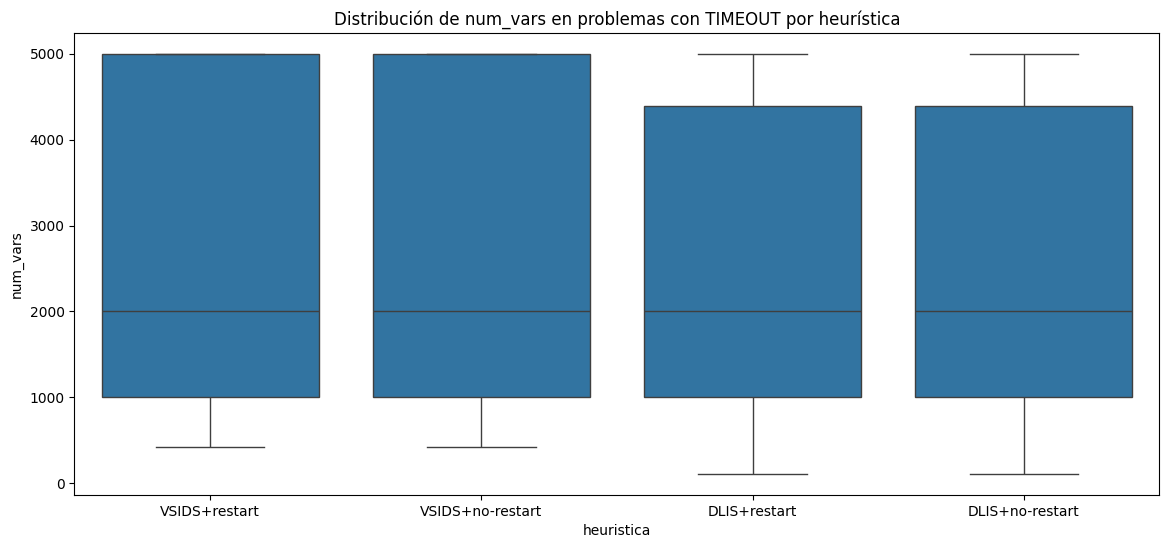
\includegraphics[width=0.8\textwidth]{Graphics/num_vars_timeout_x_heuristica.png}
    \caption{Distribuci\'on de n\'umero de variables en problemas con timeout por heur\'istica.}
    \label{fig:num-vars-timeout-x-heuristica}
\end{figure}

Por otro lado, en la figura \ref{fig:num-claus-timeout-x-heuristica} puede observarse que el n\'umero de cl\'ausulas de las instancias analizadas muestra valores elevados y gran variabilidad, con promedios entre 15.758 y 16.875 cl\'ausulas y m\'aximos por encima de 63.000 (cifras obtenidas en los experimentos). No se observan diferencias significativas entre las estrategias con DLIS o VSIDS, ni tampoco al incorporar o no el mecanismo de restart.

\begin{figure}[ht]
    \centering
    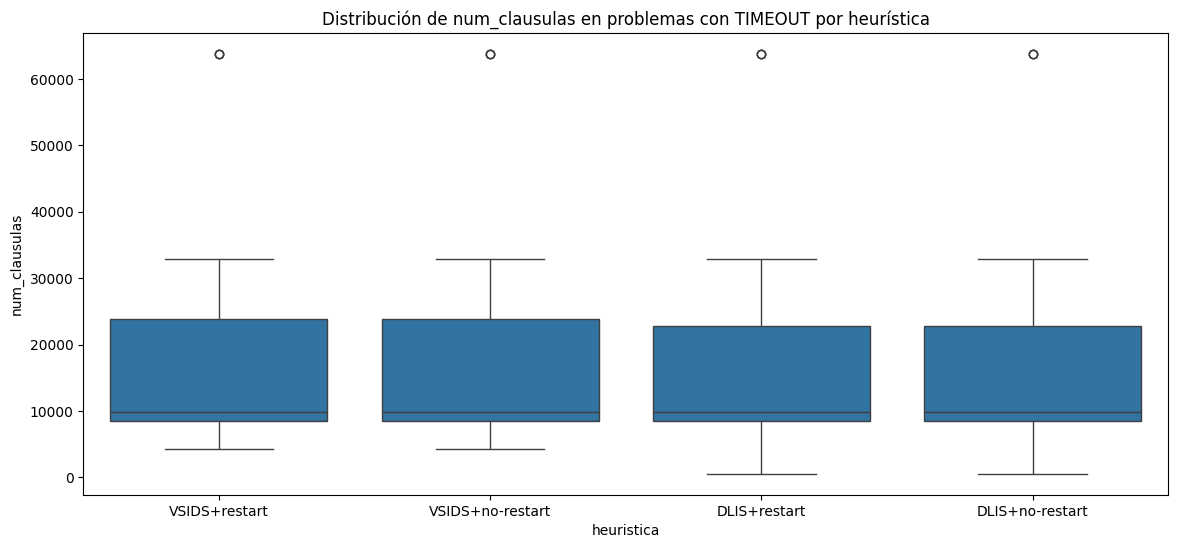
\includegraphics[width=0.8\textwidth]{Graphics/num_claus_timeout_x_heuristica.png}
    \caption{Distribuci\'on de n\'umero de cl\'ausulas en problemas con timeout por heur\'istica.}
    \label{fig:num-claus-timeout-x-heuristica}
\end{figure}

Como se muestra en \ref{fig:densidad-timeout-x-heuristica}, la densidad media se mantiene cercana a 7.4–7.7 para todas las heurísticas, con una dispersión considerable que alcanza hasta 25, lo que refleja que tanto problemas poco densos como muy densos pueden provocar fallos por tiempo.

\begin{figure}[ht]
    \centering
    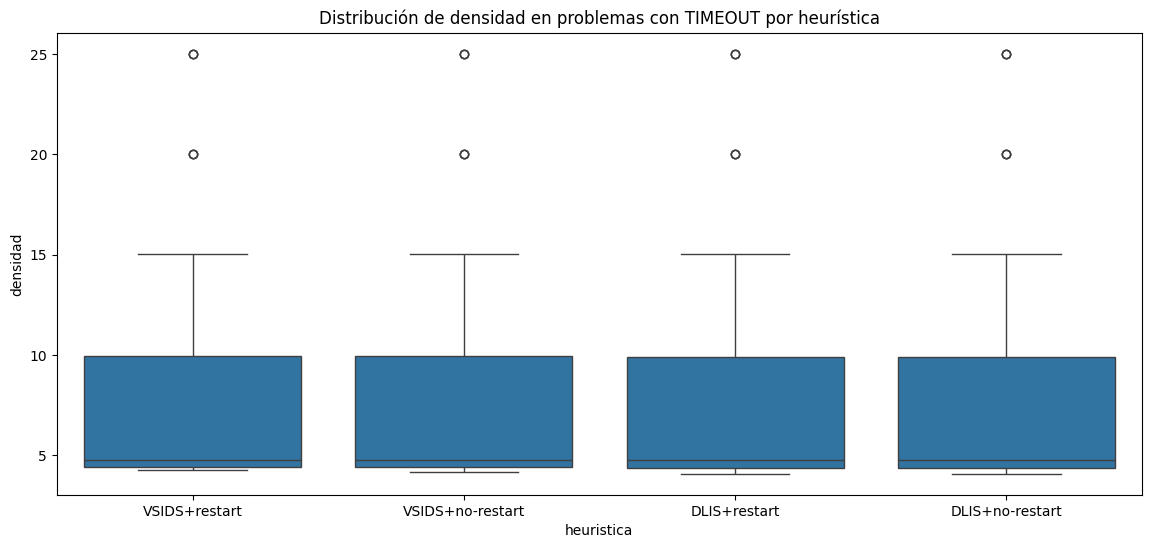
\includegraphics[width=0.8\textwidth]{Graphics/densidad_timeout_x_heuristica.png}
    \caption{Distribuci\'on de densidad en problemas con timeout por heur\'istica.}
    \label{fig:densidad-timeout-x-heuristica}
\end{figure}

En la figura \ref{fig:tamanio-prom-claus-timeout-x-heuristica} se puede apreciar que el tamaño promedio de cláusula se mantiene estable alrededor de 3, con poca variabilidad, sugiriendo que esta característica no discrimina el comportamiento de las heurísticas en cuanto a TIMEOUT.

\begin{figure}[ht]
    \centering
    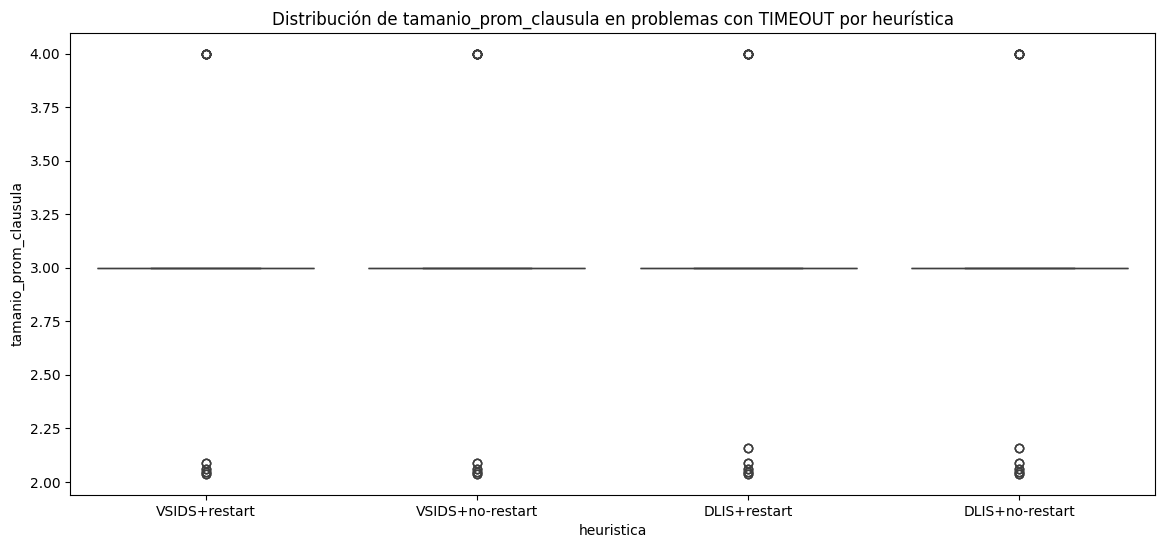
\includegraphics[width=0.8\textwidth]{Graphics/tamanio_prom_claus_timeout_x_heuristica.png}
    \caption{Distribuci\'on de tama\~no promedio de cl\'ausula en problemas con timeout por heur\'istica.}
    \label{fig:tamanio-prom-claus-timeout-x-heuristica}
\end{figure}

Por su parte, en las gr\'aficas \ref{fig:vars-pos-timeout-x-heuristica} y \ref{fig:vars-neg-timeout-x-heuristica}, se puede ver que las variables positivas y negativas, respectivamente, también muestran simetría y valores medios similares entre heurísticas, lo que implica que la polaridad de las variables no es un factor determinante en la ocurrencia de TIMEOUT.

\begin{figure}[ht]
    \centering
    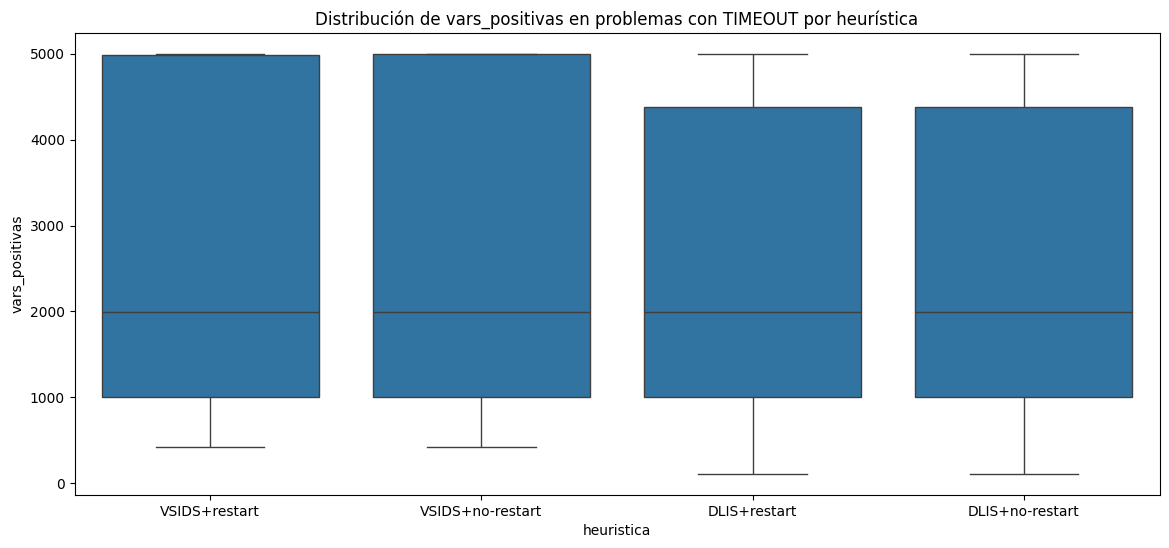
\includegraphics[width=0.8\textwidth]{Graphics/vars_pos_timeout_x_heuristica.png}
    \caption{Distribuci\'on de variables positivas en problemas con timeout por heur\'istica.}
    \label{fig:vars-pos-timeout-x-heuristica}
\end{figure}

\begin{figure}[ht]
    \centering
    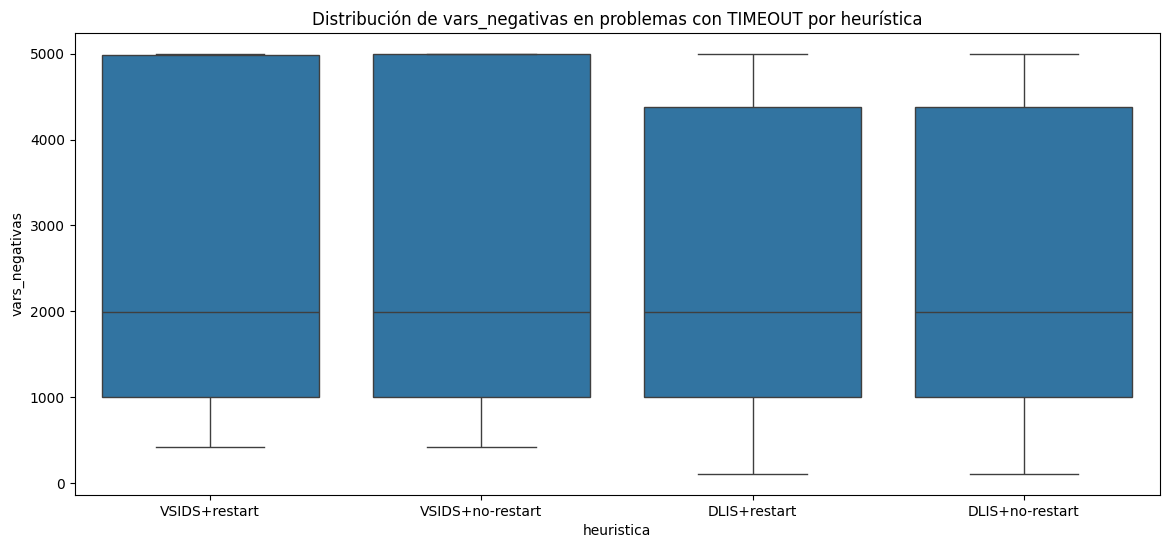
\includegraphics[width=0.8\textwidth]{Graphics/vars_neg_timeout_x_heuristica.png}
    \caption{Distribuci\'on de variables negativas en problemas con timeout por heur\'istica.}
    \label{fig:vars-neg-timeout-x-heuristica}
\end{figure}

En conjunto, estos resultados sugieren que las diferencias en el rendimiento entre heurísticas no se explican fácilmente por las características básicas de las instancias con TIMEOUT.

Las visualizaciones de caja muestran solapamientos amplios en las distribuciones de cada caracter\'istica por heur\'istica.

\subsubsection{Conteo de TIMEOUT por heur\'istica y por problema}

En las gr\'aficas \ref{fig:timeouts-x-heuristica} y \ref{fig:timeouts-x-problema} se puede observar que los problemas que tomaron mas tiempo en resolverse coinciden con los los planteados en la literatura que resultan mas dificiles de resolver a instancias SAT. Respecto a la cantidad de problemas con TIMEOUTS por heuristica, se puede apreciar que DLIS, independientemente del restart, se comporta mas lento que vsids para algunos problemas. Por su parte, vsids con restart se comporta mas lento que vsids sin restart para unas pocas instancias.

\begin{figure}[ht]
    \centering
    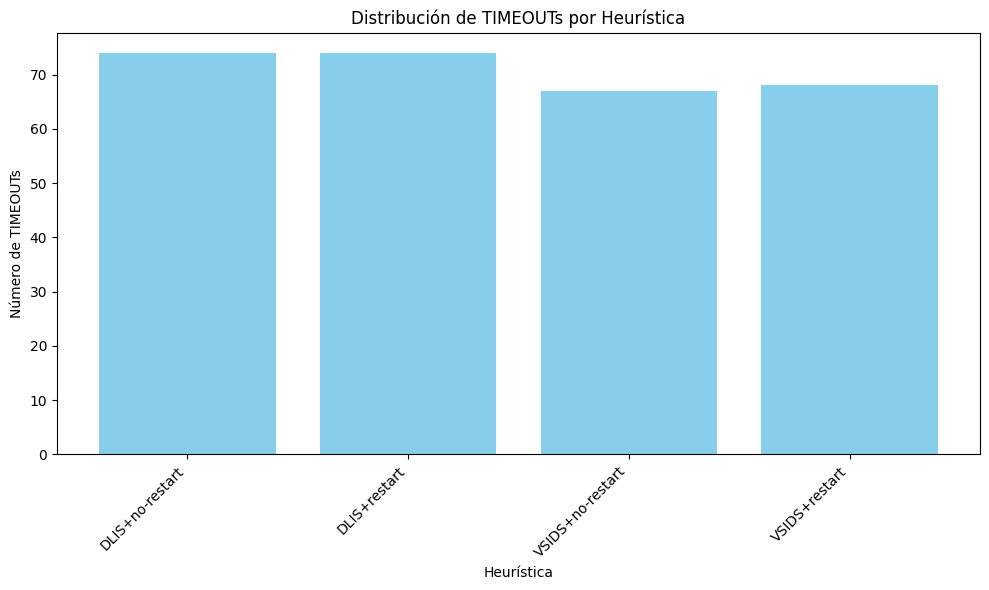
\includegraphics[width=0.8\textwidth]{Graphics/timeouts_x_heuristica.png}
    \caption{Distribuci\'on de timeouts por heur\'istica.}
    \label{fig:timeouts-x-heuristica}
\end{figure}

\begin{figure}[ht]
    \centering
    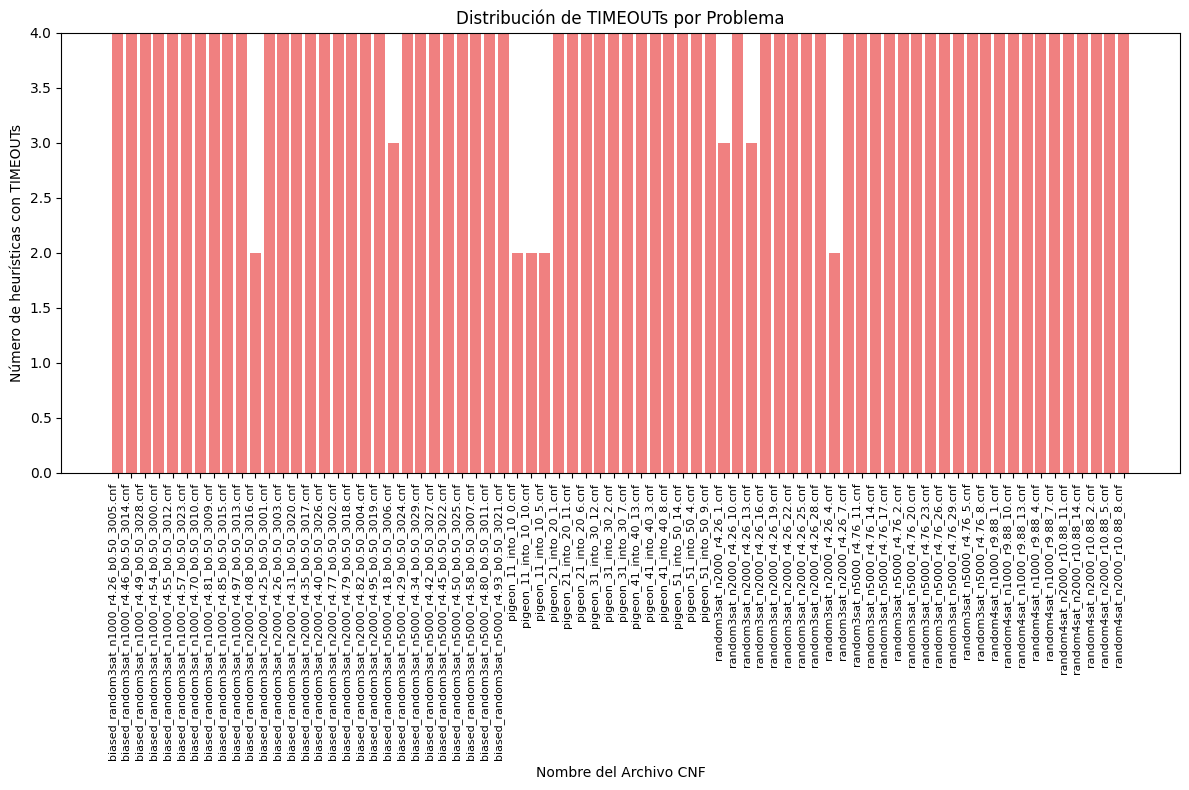
\includegraphics[width=0.8\textwidth]{Graphics/timeouts_x_problema.png}
    \caption{Distribuci\'on de timeouts por problema.}
    \label{fig:timeouts-x-problema}
\end{figure}

\subsection{An\'alisis de problemas resueltos (SATISFIABLE/UNSATISFIABLE)}

\subsubsection{Tabla resumen de RESUELTOS}
(insertar grafico que describa los resultados de la tabla filtrada por problemas resueltos)

El análisis de los problemas resueltos muestra que las instancias que concluyeron satisfactoriamente (ya sea SATISFIABLE o UNSATISFIABLE) abarcan un amplio rango de tamaños y características, desde problemas muy pequeños con 6 variables y 12 cláusulas hasta otros considerablemente más grandes con hasta 5000 variables y más de 23000 cláusulas.

Los tiempos de resolución registrados varían notablemente, desde fracciones de segundo en problemas pequeños (por ejemplo, alrededor de 0.0014 segundos en instancias con 6 variables) hasta varios segundos en problemas más complejos (por ejemplo, cerca de 9 segundos en instancias con 500 variables y alta densidad). Esto indica que, aunque el solver puede resolver eficientemente instancias pequeñas o medianas, el tiempo de cómputo crece conforme aumentan la cantidad de variables y cláusulas, así como la densidad del problema.

La presencia de las cuatro heurísticas en los resultados resueltos sugiere que todas son capaces de resolver ciertos conjuntos de problemas. Sin embargo, la diversidad en tiempos y tamaños sugiere que la heurística y la estrategia de reinicio podrían influir en la eficiencia, especialmente en problemas de mayor escala.

\subsubsection{Estad\'isticas descriptivas}


El análisis estadístico descriptivo del tiempo de resolución y las características de las instancias resueltas por cada heurística revela patrones importantes sobre el comportamiento del \textit{solver}. Estos resultados pueden apreciarse en conjunto en la gr\'afica \ref{fig:caract-tiempo-x-heuristica}.

\begin{figure}[ht]
    \centering
    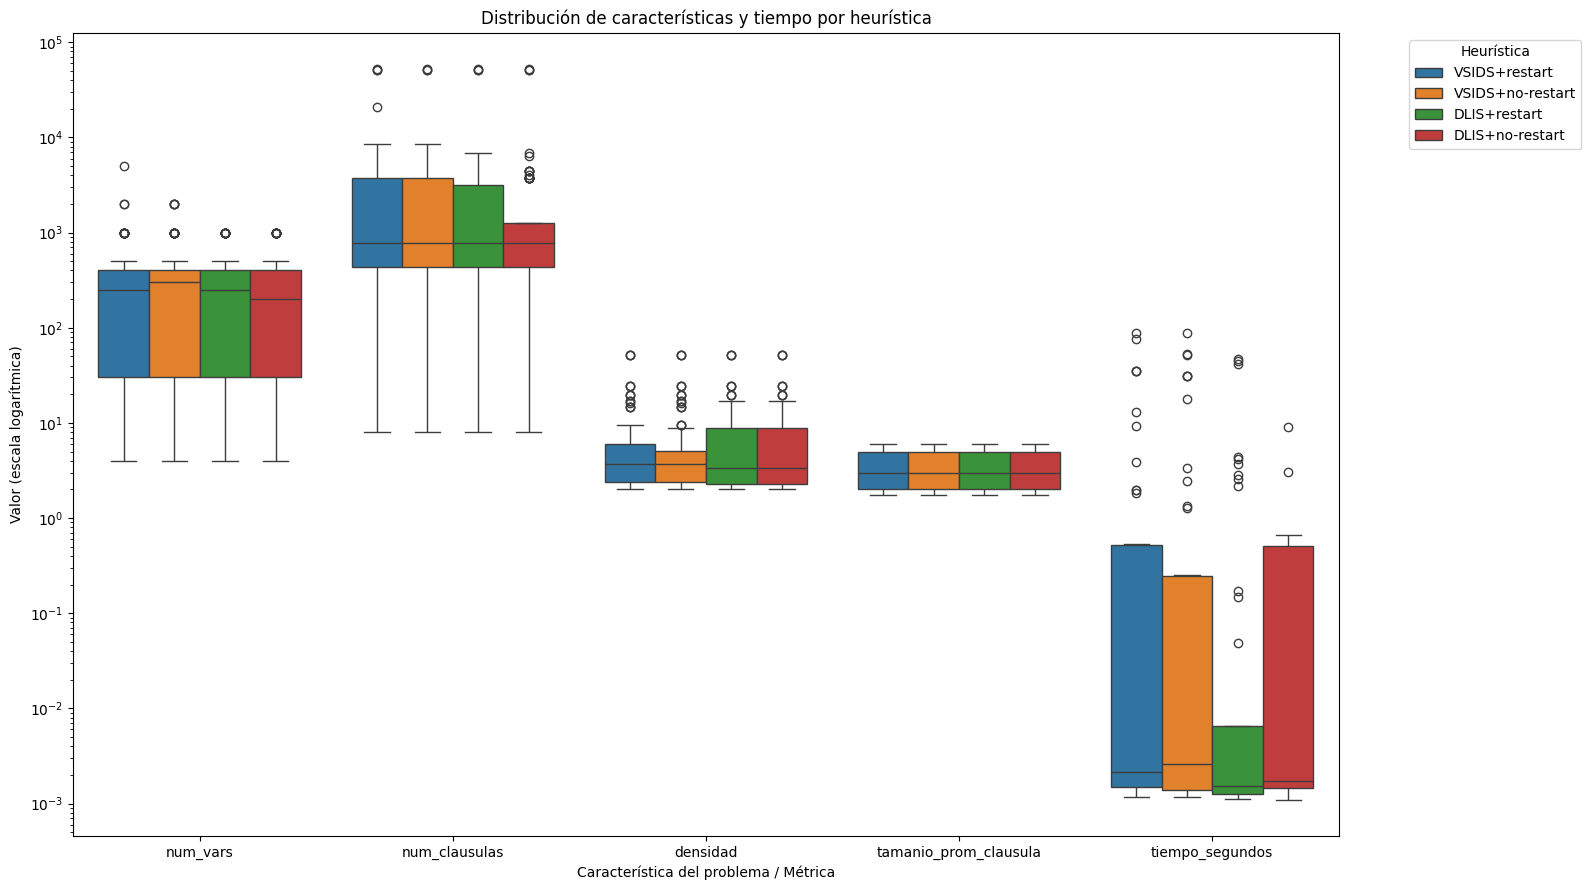
\includegraphics[width=0.8\textwidth]{Graphics/caracteristica_tiempo_x_heuristica.png}
    \caption{Distribuci\'on de caracter\'isticas y tiempo por heur\'istica.}
    \label{fig:caract-tiempo-x-heuristica}
\end{figure}


En primer lugar, se observa que las instancias resueltas por las cuatro heurísticas (DLIS+no-restart, DLIS+restart, VSIDS+no-restart y VSIDS+restart) cubren un rango amplio en tamaño, con número de variables promedio entre 322 y 403, y máximos que alcanzan hasta 2000 o incluso 5000 variables en el caso de VSIDS+restart. La cantidad de cláusulas también presenta gran dispersión, con medias cercanas a 3100–3400 y máximos que superan las 50,000, lo que indica que el solver puede manejar problemas desde muy pequeños hasta instancias complejas. La densidad promedio se mantiene alrededor de 7,2 a 7,4, con valores máximos muy altos (hasta 51.9), reflejando diversidad en la estructura de los problemas.

En cuanto al tiempo de resolución, se evidencia una marcada diferencia entre heurísticas: DLIS+no-restart presenta el tiempo medio más bajo (~0.37 s), seguido por DLIS+restart (~3.13 s), mientras que VSIDS+no-restart y VSIDS+restart muestran tiempos medios más elevados, cerca de 4.98 y 4.98 segundos respectivamente, con alta variabilidad (desviaciones estándar muy grandes y máximos que superan los 80 segundos). Esta dispersión sugiere que aunque VSIDS puede ser eficiente en muchos casos, también enfrenta problemas que requieren tiempos significativamente mayores. Además, la mediana del tiempo para todas las heurísticas es muy baja (en el orden de milisegundos), indicando que la mayoría de las instancias se resuelven rápidamente, pero existen casos atípicos que prolongan el tiempo promedio.

El tamaño promedio de cláusula es similar entre heurísticas, alrededor de 3.4, y las variables positivas y negativas mantienen valores simétricos, lo que indica que estas características no explican las diferencias en tiempo.

En conjunto, estos resultados sugieren que la elección de heurística impacta significativamente el tiempo de resolución en ciertos problemas, especialmente en instancias grandes o complejas, y que VSIDS puede tener mayor variabilidad en rendimiento.

\subsection{Porblemas RESUELTOS vs TIMEOUT}

\subsubsection{An\'alisis de multicolinealidad}

\begin{figure}[ht]
    \centering
    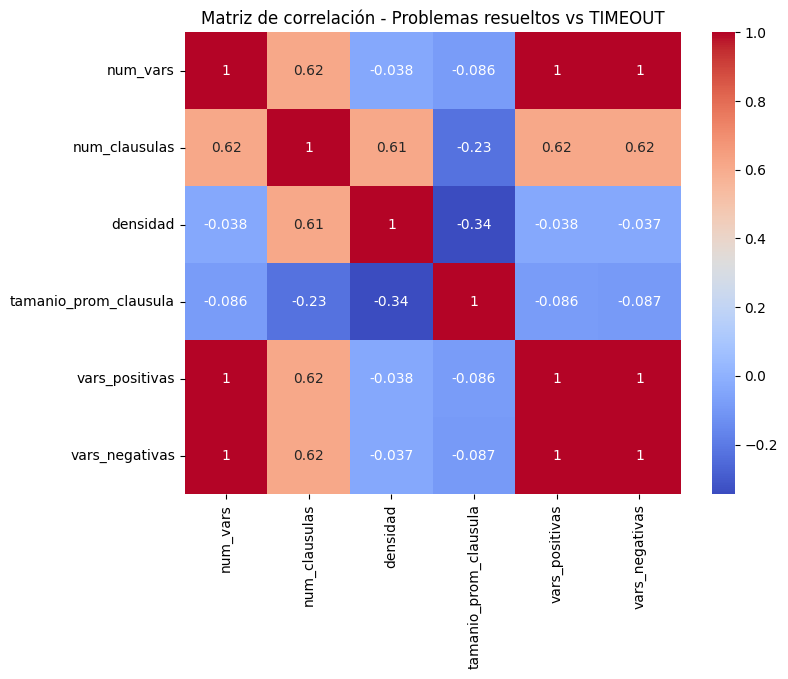
\includegraphics[width=0.8\textwidth]{Graphics/correlation_matrix_solveds_vs_timeouts.png}
    \caption{Matriz de correlaci\'on - Problemas resueltos vs TIMEOUTS.}
    \label{fig:correlation-matrix-solved-vs-timeout}
\end{figure}

Como se puede apreciar en la matriz de correlaci\'on \ref{fig:correlation-matrix-solved-vs-timeout}, entre las variables num\_vars y vars\_positivas y vars\_negativas, existe correlaci\'on perfecta ($r=1$). Adem\'as, existe una correlaci\'on moderada entre las variables num\_clausulas con vars\_negativas, vars\_positivas, num\_vars y densidad). Luego, es necesario reducir el conjunto de caracter\'isticas, quedando  el siguiente: \texttt{caracteristicas\_reducidas = [`num\_vars', `densidad', `tamanio\_prom\_clausula'] \footnote{Estos son los mismos nombres con los que se guardaron los datos}}.

\begin{figure}[ht]
    \centering
    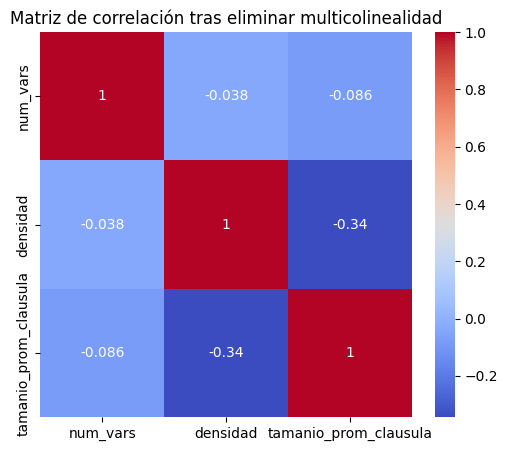
\includegraphics[width=0.8\textwidth]{Graphics/correlation_matrix_after_delete_multicol.png}
    \caption{Matriz de correlaci\'on tras eliminar multicolinealidad.}
    \label{fig:correlation-matrix-after-delete-multicol}
\end{figure}

Como se muestra en la matriz \ref{fig:correlation-matrix-after-delete-multicol}, se elimin\'o las correlaciones moderadas y severas.

\subsubsection{Comparaci\'on de caracter\'isticas entre RESUELTOS Y TIMEOUTs}

Al realizar el test de normalidad de Shapiro-Wilk se obtuvo los resultados mostrados en \ref{fig:test-shapiro-wilk}:


\begin{figure}[ht]
    \centering
    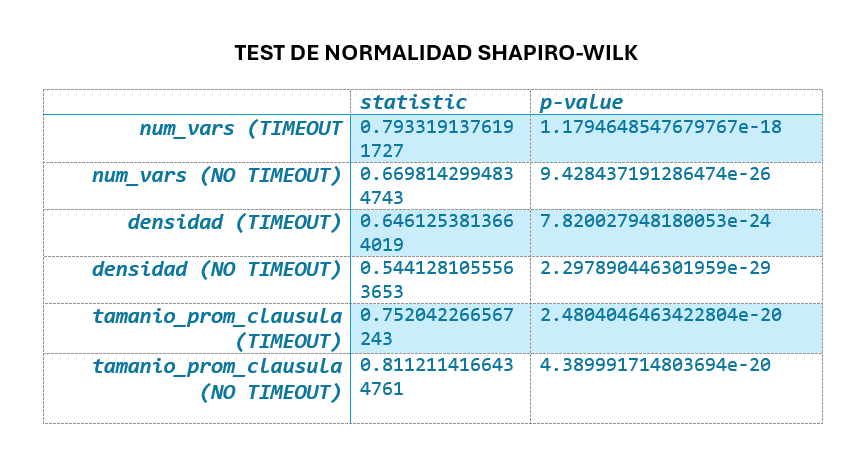
\includegraphics[width=0.8\textwidth]{Graphics/test_shapiro_wilk.png}
    \caption{Test de normalidad Shapiro-Wilk.}
    \label{fig:test-shapiro-wilk}
\end{figure}

Este an\'alisis mostrado en la tabla \ref{fig:test-shapiro-wilk} revela que ninguna de estas características sigue una distribución normal en los grupos de instancias que terminaron en TIMEOUT ni en las que fueron resueltas. Esto se evidencia en los valores de p muy bajos (todos menores a 0.05, incluso extremadamente cercanos a cero), lo que permite rechazar la hipótesis nula de normalidad para cada variable en ambos grupos. En concreto, los estadísticos de Shapiro oscilan entre aproximadamente 0.54 y 0.81, y los p-valores indican una desviación significativa de la normalidad.

Luego, para comparar estas características entre instancias con y sin TIMEOUT no es apropiado utilizar pruebas paramétricas basadas en la normalidad, como el t-test, sino que se deben emplear métodos no paramétricos, por ejemplo la prueba de Mann-Whitney, cuyo resultado se presenta a continuaci\'on. 

\subsubsection{Prueba Mann-Whitney U}

\begin{figure}[ht]
    \centering
    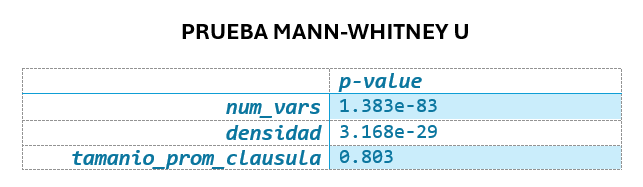
\includegraphics[width=0.8\textwidth]{Graphics/prueba_mann_whitney_u.png}
    \caption{Prueba Mann-Whitney U.}
    \label{fig:prueba-mann-whitney-u}
\end{figure}

Como se muestra en \ref{fig:prueba-mann-whitney-u}, la prueba muestra resultados concluyentes sobre las diferencias entre las instancias que terminaron en TIMEOUT y las que fueron resueltas. Estos, visualizarse de igual forma mediante las gr\'aficas \ref{fig:dist-man-whitney}.


\begin{figure}[ht]
    \centering
    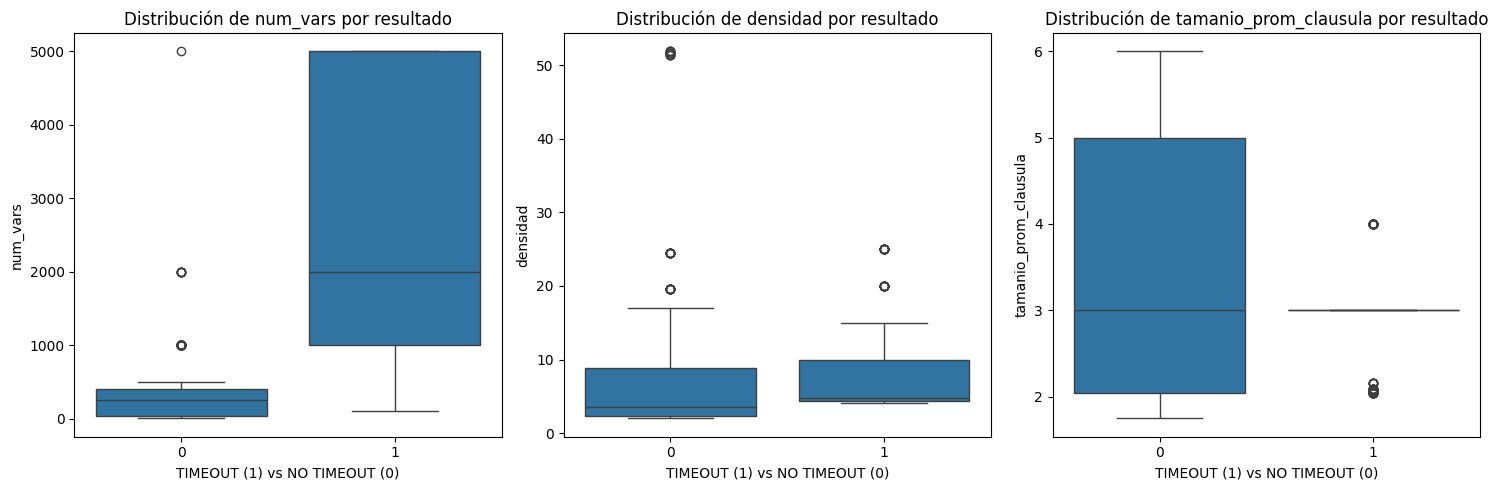
\includegraphics[width=0.8\textwidth]{Graphics/man_whitney.png}
    \caption{Distribuciones de prueba Mann-Whitney U por resultados.}
    \label{fig:dist-man-whitney}
\end{figure}

Para las variables n\'umero de variables y densidad, los valores p son extremadamente bajos (1.383e-83 y 3.168e-29 respectivamente), lo que indica diferencias estadísticamente significativas entre ambos grupos en estas características. Esto sugiere que tanto el tamaño del problema como su densidad influyen fuertemente en la probabilidad de que un problema termine en TIMEOUT.

En contraste, para el tamaño promedio de cláusula el p-valor es alto (0.803), lo que implica que no hay evidencia suficiente para afirmar que esta característica difiera entre problemas con y sin TIMEOUT.

Estos resultados confirman que las variables relacionadas con la escala y complejidad estructural del problema (num\_vars y densidad) son factores determinantes en el rendimiento del \textit{solver}, mientras que el tamaño promedio de las cl\'ausulas no parece ser un factor discriminante en la ocurrencia de TIMEOUT.

En consecuencia, para modelar o predecir la probabilidad de TIMEOUT conviene priorizar las variables num\_vars y densidad, y descartar o tratar con menor peso el tamaño promedio de cláusula.

\subsubsection{Regresi\'on log\'istica: ¿Qué caracter\'isticas predicen TIMEOUT?}

Tras efectuar la regresi\'on se obtuvieron los siguientes resultados \ref{fig:regresion-logistica}:

\begin{figure}[ht]
    \centering
    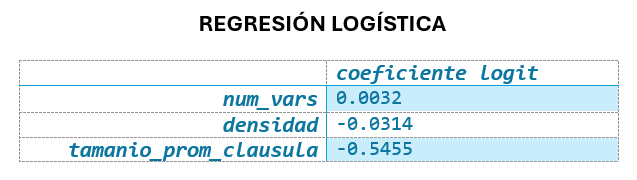
\includegraphics[width=0.8\textwidth]{Graphics/regresion_logistica.png}
    \caption{Regresi\'on log\'istica.}
    \label{fig:regresion-logistica}
\end{figure}

Con base en estos resultados de la tabla \ref{fig:regresion-logistica} , el modelo ofrece una interpretación clara sobre la influencia de cada característica en la probabilidad de que un problema no se resuelva en el tiempo límite.

El coeficiente positivo para num\_vars (0.0032) indica que a medida que aumenta el número de variables, la probabilidad de TIMEOUT también incrementa, lo cual es consistente con la intuición y los análisis descriptivos previos que mostraron que problemas más grandes tienden a ser más difíciles de resolver. 

Por otro lado, los coeficientes negativos para densidad (-0.0314) y especialmente para tamaño promedio de cláusula (-0.5455) sugieren que, manteniendo constante el número de variables, un aumento en estas características está asociado con una menor probabilidad de TIMEOUT. En particular, el tamaño promedio de cláusula tiene un efecto considerablemente más fuerte en sentido negativo, lo que podría indicar que cláusulas más largas o complejas, dentro del rango observado, facilitan la resolución o están asociadas a problemas menos propensos a agotar el tiempo.

Estos signos y magnitudes reflejan que la complejidad estructural del problema no se reduce solo al tamaño, sino que la forma en que las cláusulas están construidas también impacta el rendimiento del solver. En conjunto, el modelo confirma y cuantifica las tendencias observadas en análisis estadísticos previos, y ofrece una base para predecir y ajustar heurísticas en función de las características del problema para minimizar la ocurrencia de TIMEOUT.

\subsection{Rendimiento de las heur\'isticas en problemas resueltos}
Para los an\'alisis estad\'isticos en esta secci\'on se incluy\'o la variable tiempo, que e=indica en seg cu\'anto tard\'o el \textit{solver} en dar una soluci\'on.

\subsubsection{Correlaci\'on de Spearman}
Se obtuvo los siguientes resultados \ref{fig:correlacion-spearman}:

\begin{figure}[ht]
    \centering
    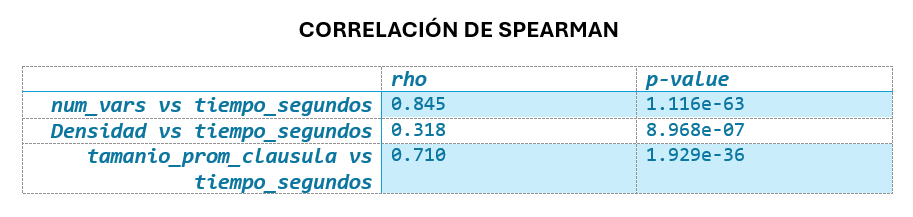
\includegraphics[width=0.8\textwidth]{Graphics/correlacion_spearman.png}
    \caption{Correlaci\'on de Spearman.}
    \label{fig:correlacion-spearman}
\end{figure}

Los resultados que se muestran en la tabla \ref{fig:correlacion-spearman} an\'alisis revela asociaciones significativas y de distinta intensidad.

La variable número de variables muestra una correlación muy fuerte y positiva con el tiempo de resolución (rho = 0.845, p < 0.001), indicando que a mayor tamaño del problema, mayor es el tiempo requerido para resolverlo, lo cual es coherente con la complejidad esperada en problemas SAT.

La densidad presenta una correlación positiva moderada (rho = 0.318, p < 0.001), lo que sugiere que problemas con mayor densidad de cláusulas por variable tienden a requerir más tiempo, aunque este efecto es menos pronunciado que el del tamaño.

Por último, el tamaño promedio de cl\'ausula tambi\'en exhibe una correlación fuerte positiva (rho = 0.710, p < 0.001), indicando que cláusulas más largas o complejas están asociadas con un aumento significativo en el tiempo de resolución.

Estos resultados confirman que tanto la escala del problema como su estructura influyen en el rendimiento del solver, siendo el número de variables el factor más determinante, seguido por la complejidad de las cláusulas y la densidad. 

\subsubsection{Kruskal-Wallis: ¿El tiempo difiere entre heurísticas para un mismo tipo de problema?}


\begin{figure}[ht]
    \centering
    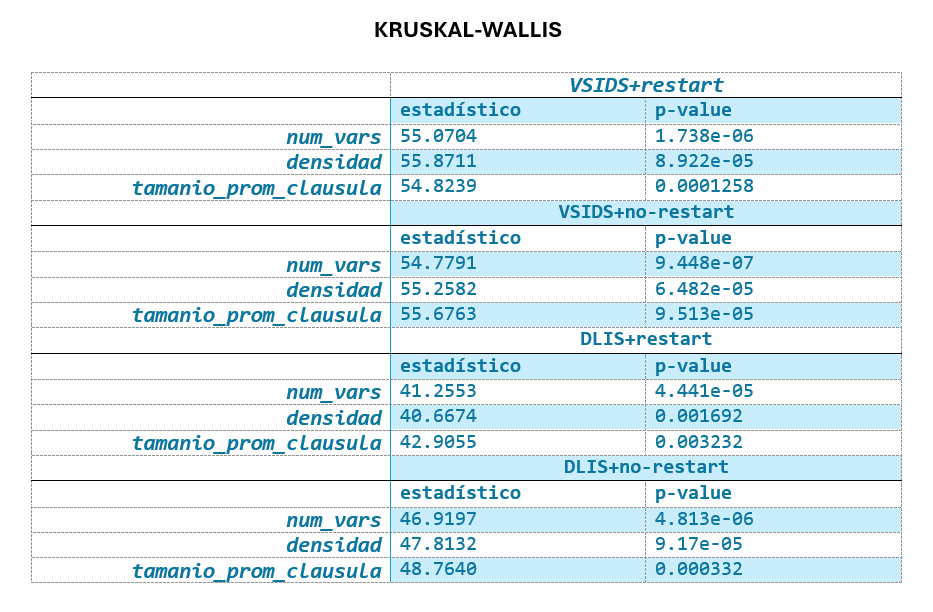
\includegraphics[width=0.8\textwidth]{Graphics/kruskal_wallis.png}
    \caption{Kruskal-Wallis.}
    \label{fig:kruskal-wallis}
\end{figure}


Dados los siguientes resultados mostrados en la tabla \ref{fig:kruskal-wallis}, se tiene que el análisis mediante la prueba no paramétrica de Kruskal-Wallis aplicado a la variable transformada del tiempo de resolución (logaritmo natural del tiempo más uno) para cada heurística y característica del problema revela diferencias estadísticamente significativas en todos los casos evaluados.

Para las cuatro heurísticas (VSIDS+restart, VSIDS+no-restart, DLIS+restart y DLIS+no-restart), las variables número de variables, densidad y tamaño promedio de cláusula muestran valores de estadístico elevados y p-valores muy bajos (todos menores a 0.005), lo que indica que la distribución del tiempo de resolución difiere significativamente entre los distintos grupos definidos por cada una de estas características. Esto implica que, independientemente de la heurística utilizada, las propiedades estructurales del problema impactan de forma relevante en el rendimiento temporal del \textit{solver}.

La consistencia de estos resultados a través de todas las heurísticas sugiere que la influencia de estas variables es robusta y generalizable, reafirmando su importancia en el análisis y modelado del comportamiento del solver SAT. Además, el uso del logaritmo del tiempo como variable respuesta ayuda a mitigar la influencia de valores extremos y facilita la detección de diferencias significativas en la mediana y distribución del tiempo. 

\subsubsection{Pruebas post hoc con test de Dunn}

Para estas pruebas se obtuvieron los resultados mostrados en las tablas \ref{fig:test-dunn-vsids-restart}, \ref{fig:test-dunn-vsids-no-restart}, \ref{fig:test-dunn-dlis-restart} y \ref{fig:test-dunn-dlis-no-restart}:

\begin{figure}[ht]
    \centering
    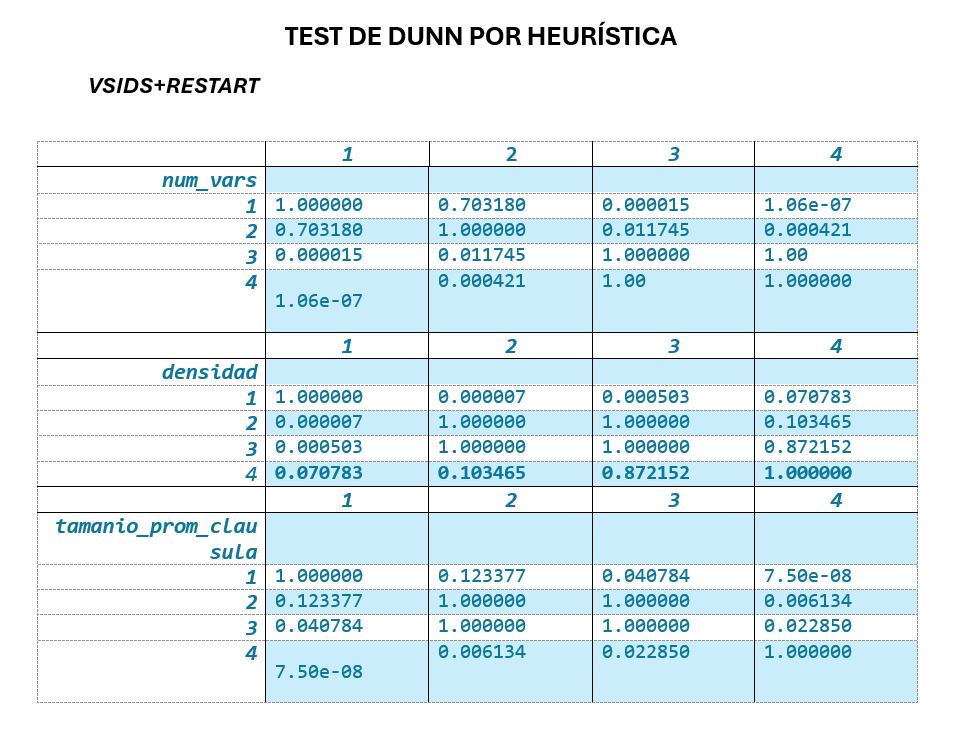
\includegraphics[width=0.8\textwidth]{Graphics/test_dunn_vsids_restart.png}
    \caption{Test Dunn por cuartiles para VSIDS con restart.}
    \label{fig:test-dunn-vsids-restart}
\end{figure}

\begin{figure}[ht]
    \centering
    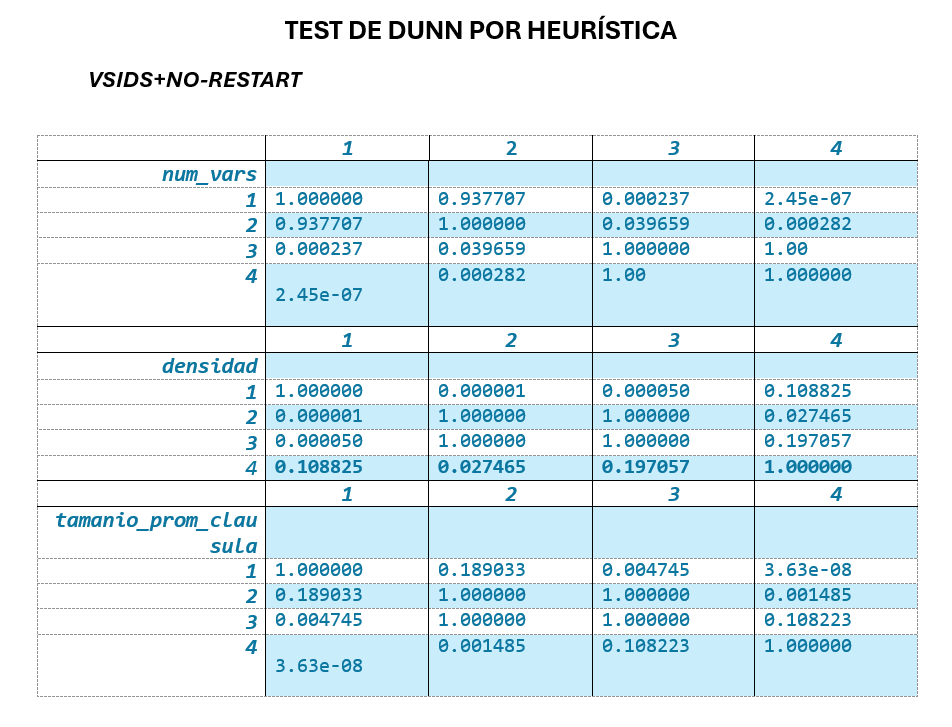
\includegraphics[width=0.8\textwidth]{Graphics/test_dunn_vsids_no_restart.png}
    \caption{Test Dunn por cuartiles para VSIDS sin restart.}
    \label{fig:test-dunn-vsids-no-restart}
\end{figure}

\begin{figure}[ht]
    \centering
    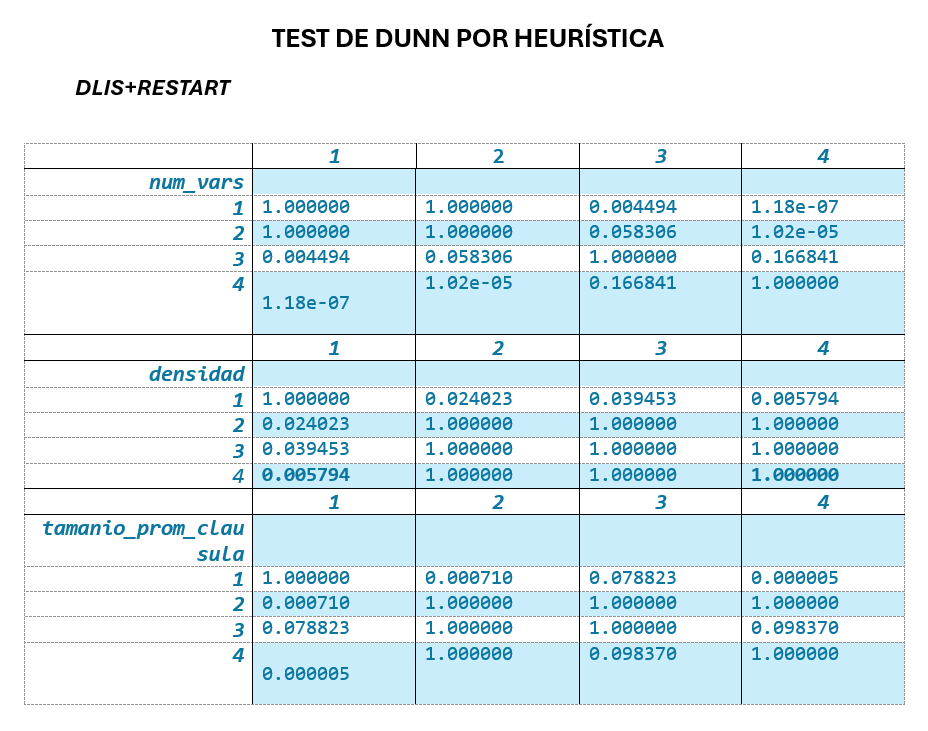
\includegraphics[width=0.8\textwidth]{Graphics/test_dunn_dlis_restart.png}
    \caption{Test Dunn por cuartiles para DLIS con restart.}
    \label{fig:test-dunn-dlis-restart}
\end{figure}

\begin{figure}[ht]
    \centering
    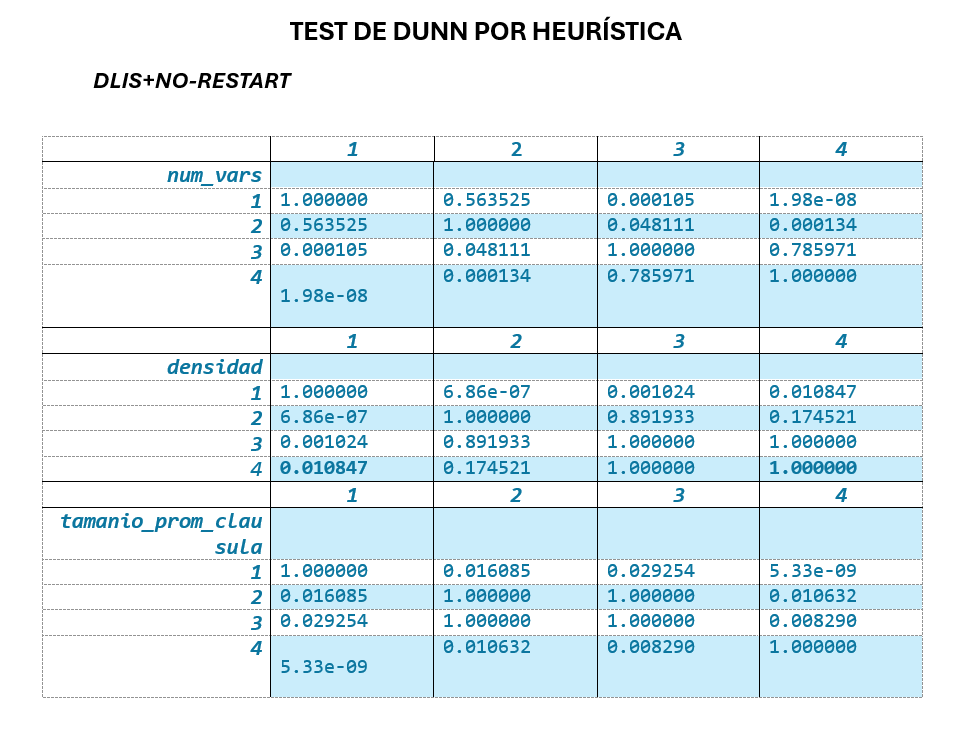
\includegraphics[width=0.8\textwidth]{Graphics/test_dunn_dlis_no_restart.png}
    \caption{Test Dunn por cuartiles para DLIS csin restart.}
    \label{fig:test-dunn-dlis-no-restart}
\end{figure}

El test post-hoc de Dunn aplicado por cuartiles (grupos definidos con ranking para evitar empates) para cada heurística y variable seleccionada permite identificar con precisión entre qué grupos existen diferencias significativas en el tiempo de resolución (logaritmo del tiempo).

En general, para la variable ``número de variables'', se observan diferencias altamente significativas entre los cuartiles extremos (por ejemplo, grupo 1 vs. 4) en todas las heurísticas, con p-valores muy bajos (p < 0.001), lo que confirma que problemas más grandes requieren tiempos significativamente mayores para resolverse. En los grupos intermedios, las diferencias son menos consistentes pero también aparecen comparaciones significativas, evidenciando una relación gradual entre tamaño y tiempo. 

Para la densidad, los resultados muestran diferencias significativas principalmente entre los cuartiles más bajos y más altos, aunque en algunos casos los grupos intermedios no difieren tanto, indicando que la densidad afecta el tiempo pero con menor fuerza y de manera menos lineal que el tamaño.

En cuanto al tamaño promedio de cláusula, también se detectan diferencias significativas entre los extremos, especialmente entre el primer y cuarto cuartil, y en varios casos entre grupos adyacentes, lo que sugiere que esta variable influye en el rendimiento, aunque su efecto puede ser más sutil o no monotónico.

La consistencia de estos patrones a lo largo de todas las heurísticas refuerza la importancia de estas características para explicar la variabilidad en el tiempo de resolución.

